% APLAS 2021: Regular research papers should not exceed 18 pages in
% the Springer LNCS format(LaTeX template), including bibliography and
% figures.
% Lightweight double-blind: Author names and institutions must be
% omitted and References to the authors’ own related work should be in
% the third person 
%
\documentclass[runningheads]{llncs}
\pdfoutput=1
%\usepackage[english]{babel}
\usepackage[utf8]{inputenc}
\usepackage{amsmath}
\usepackage{amssymb}
%\usepackage{graphicx}
%\usepackage[colorinlistoftodos]{todonotes}
\usepackage{mathpartir}
\usepackage{graphicx}
%\usepackage{fixme}
%\usepackage{xcolor}
\usepackage{hyperref}
\usepackage{listings}
\lstdefinelanguage{michelson}{
  % basicstyle=\ttfamily,
  basicstyle=\fontsize{8}{9.6}\selectfont,
  morekeywords={parameter,storage,or,unit,mutez,pair,bool,address}, sensitive=false,
  morecomment=[l]{\#},
  morecomment=[s]{/*}{*/},
  morestring=[b]",
}
\lstset{
  language=Caml,
  captionpos=b,
  aboveskip=-\smallskipamount,
  belowskip=-\smallskipamount,
  belowcaptionskip=0pt,
  basicstyle=\fontsize{8}{9.6}\selectfont,
  morekeywords={val}
}

%% structure
\newcommand{\Angle}[1]{\langle#1\rangle}

%% values
\newcommand\SUNIT{\textbf{()}}
\newcommand{\TRUE}{\textbf{True}}
\newcommand{\FALSE}{\textbf{False}}

%% names
\newcommand{\ALS}{\textbf{als}}
\newcommand{\PAK}{\textbf{pak}}
\newcommand{\PUK}{\textbf{puk}}
\newcommand{\PKH}{\textbf{pkh}}
\newcommand{\PUH}{\textbf{puh}}
\newcommand{\CODE}{\textbf{code}}
\newcommand{\BAL}{\textbf{bal}}
\newcommand{\COU}{\textbf{cou}}
\newcommand{\STORAGE}{\textbf{storage}}
\newcommand{\OP}{\textbf{op}}
\newcommand{\OPH}{\textbf{oph}}
\newcommand{\TIME}{\textbf{t}}
\newcommand{\CONTRACTORS}{\textbf{T}}
\newcommand{\PENDING}{\textbf{P}}
\newcommand{\ACCEPTED}{\textbf{A}}
\newcommand{\MANAGERS}{\textbf{K}}
%% operations
\newcommand{\TRANSFER}[5][\SUNIT]{\text{transfer $#2$ from $#3$ to $#4$ arg $#1$ fee $#5$}}
\newcommand{\ORIGINATE}[6]{\text{originate contract $#1$ transferring $#2$ from $#3$ running $#4$ init $#5$ fee $#6$}}
\newcommand{\NTEZ}{\textbf{n}}
\newcommand{\MTEZ}{\textbf{m}}
\newcommand{\ID}{\textbf{id}}
\newcommand\STRING{\textbf{s}}
%% queries
\newcommand{\QRY}{\textbf{qry}}
\newcommand{\GETBALANCE}[1]{\text{get balance for $#1$}}
\newcommand{\GETSTATUS}[1]{\text{get status for $#1$}}
\newcommand{\GETSTORAGE}[1]{\text{get contract storage $#1$}}
\newcommand{\GETCODE}[1]{\text{get code for $#1$}}
\newcommand{\GETPUBLICKEY}[1]{\text{get public key for $#1$}}
\newcommand{\GETCOUNTER}[1]{\text{get counter for $#1$}}

\newcommand{\ACCOUNTS}{\textbf{C}}
\newcommand{\OPERATIONS}{\textbf{O}}
\newcommand{\CONTRACTS}{\textbf{S}}

\newcommand{\NODE}{\textbf{N}}
\newcommand{\BLOCKCHAIN}{\textbf{B}}

%% functions
\newcommand{\CHECKACC}{\textup{checkAcc}}
\newcommand{\CHECKID}{\textup{checkId}}
\newcommand{\CHECKBAL}{\textup{checkBal}}
\newcommand{\CHECKCOU}{\textup{checkCou}}
\newcommand{\CHECKPUB}{\textup{checkPub}}
\newcommand{\UPDATECOU}{\textup{updateCou}}

\newcommand{\GENERATEOPH}{\textup{generateOph}}

%% transition relations
\newcommand{\NodeTrans}{\longrightarrow_N}
\newcommand{\SystemTrans}{\longrightarrow}



\begin{document}
%
\title{Assertion Contracts}
%
%\titlerunning{Abbreviated paper title}
% If the paper title is too long for the running head, you can set
% an abbreviated paper title here
%
%\author{Thi Thu Ha Doan\orcidID{0000-0001-7524-4497}\and Peter Thiemann\orcidID{0000-0002-9000-1239}}

%
%\authorrunning{Ha Doan, P. Thiemann}
% First names are abbreviated in the running head.
% If there are more than two authors, 'et al.' is used.
%
%\institute{University of Freiburg, Germany \\ \email{\{doanha,thiemann\}@informatik.uni-freiburg.de}
%}
%
\maketitle              % typeset the header of the contribution
%
\begin{abstract}
 
\keywords{}
\end{abstract}

%
%
%
\section{Introduction}
\label{sec:introduction}
Every computation performed by a Smart Contract on the blockchain generates costs. Each
unit of computation and each unit of storage used by an algorithm must be paid for. To
avoid this cost, an application might perform some computation away from the blockchain
(i.e., off-chain) and submit the result as a parameter to a contract on the
blockchain. Typically, such a computation asserts certain properties of the 
submitted parameter. 

However, this approach raises the issue that on the one hand the contract should take
advantage of the offchain computation and assume that the submitted parameter has
these properties, but on the other hand, the off-chain computation might be wrong and
submit illegal parameters. So, we need a mechanism that checks the validity of the
assumptions before the contract starts executing.

As an example, consider a contract that takes a prime number as a parameter.
\begin{lstlisting}[numbers=none]
contract Example {
  function (int p) public {
    // assume p is prime
    ...
  }
}
\end{lstlisting}
This assumption can be expressed with an explicit assertion in predicate logic.
\begin{gather}\label{eq:5}
  (\forall n) (2 \le n \le \sqrt p) \Rightarrow (p \mathbin{\%} n) \ne 0
\end{gather}
To test the validity of this assumption requires a loop in the contract, but the test would take
$O(\sqrt p)$ time (assuming constant time for computing the remainder) and thus produce extra cost
linear in $\sqrt p$ accordingly. 
However, we could do better by recruiting the validators of the contract for a distributed
effort to find a counterexample. To this end, we consider the negation of the assertion.
\begin{gather}\label{eq:4}
  (\exists n) (2 \le n \le \sqrt p) \wedge (p \mathbin{\%} n) = 0
\end{gather}
This assertion can be checked pointwise by having each validator independently choose a
random $n$ fulfilling $2 \le n \le 
\sqrt p$ and checking whether $(p \mathbin{\%} n) = 0$. If the remainder is $0$, the
validator found a counterexample, posts its veto to the P2P net, and stops further
exection. Otherwise, it accepts $p$ knowing that other points will be checked by other
validators.

In this scenario, each validator only needs to be paid to generate a random number and
perform a division, which is a constant cost independent from $p$.

Of course, this validation is only probabilistic, so its effectiveness depends on the
number of validators. One could say that the community of validators implements a Bloom
filter for the set of primes: if a value $p$ is rejected it is certainly not a prime (because
there exists a counterexample); if a value $p$ is not rejected it is prime with a
probability that depends on $p$ and the number of validators. 

As another example, consider a contract that takes a sorted array of integers.
\begin{lstlisting}[numbers=none]
contract Sorted {
  function find (int[50] a, int v) public {
    // assume a is sorted
  }
}
\end{lstlisting}
The explicit assertion would be
\begin{gather}\label{eq:1}
  (\forall k) (0\le k <49) \Rightarrow a[k] \le a[k+1]
\end{gather}
While we can check this contract in $O(1)$ time, the constant factor is big! So we
consider its negation.
\begin{displaymath}
  (\exists k) (0\le k <49) \wedge a[k] > a[k+1]
\end{displaymath}
Again, we can have every validator generate a random number $k$. If the
condition is true for such $k$, then the validator found a counterexample for the sortedness
of the array. Otherwise, the validator relies on the other validators to check
different numbers.

To obtain an estimate of the number of validators needed to find a counterexample with
high probibility, 
let's assume the array is unsorted only at position $0$, the size of the array is $n$,
and the number of validators is $m$. Each validator independently has a probability of
$1/n$ to detect the problem and thus probability $\frac{n-1} n$ not to detect the
problem. Hence, if we assume that each $k$ is chosen independenty from a uniform distribution,
the probability that no validator checks at
position $0$ converges to $0$ as the number of validators approaches infinity.
\begin{displaymath}
  \lim_{m\to\infty}\frac{(n-1)^m}{n^m}
  = \lim_{m\to\infty} \left(\frac{n-1}{n}\right)^m
  = 0
\end{displaymath}

In Dafny (citation) \url{https://rise4fun.com/Dafny/tutorialcontent/guide#h29} you can
write
\begin{lstlisting}
forall j, k :: 0 <= j < k < a.Length ==> a[j] <= a[k]
\end{lstlisting}
to express that an array is sorted. This predicate is equivalent to the one given in
\eqref{eq:1}, but it might be more challenging to test. Its negation is
\begin{gather}
  \label{eq:2}
  (\exists j, k ) (0\le j< k < |a|) \wedge a[j] > a[k]
\end{gather}
So we'd have to generate two random numbers $j$ and $k$ such that the condition $0 \le
j < k < |a|$ is fulfilled.


Another condition that might be tested on an array is the heap condition
\begin{gather}
  \label{eq:3}
  (\forall i) (0 \le i < \lfloor|a|/2\rfloor) \Rightarrow a[i] \le a[2i+1] \wedge (2i+2
  < |a| \Rightarrow a[i] \le a[2i+2])
\end{gather}
\section{Primaries}
\label{sec:primaries}

\subsection{Smart Contract}
\label{subsec:smart-contract}

\subsection{Assertion Problem}
\label{subsec:problem}




\section{Distributed Assertion Protocol}
\label{sec:approach}
We propose an assertion verification approach for smart contracts. When a function is called with a parameter that needs to be verified, an assertion and its negation form are created for that parameter. The idea underlying our approach is that the assertion is distributed to be verified by validators. During the distribution, each validator strives to find a counterexample for the assertion. Each of these validators then checks only a random point or a small finite set  in the range of the parameter. Considering the example where a parameter $p$ is a prime number, the assertion in predicate logic for the parameter is 
\begin{gather}\label{eq:3a}
  (\forall n) (2 \le n \le \sqrt p) \Rightarrow (p \mathbin{\%} n) \ne 0
\end{gather}


\noindent and its negation form is 

\begin{gather}\label{eq:3b}
  (\exists n) (2 \le n \le \sqrt p) \wedge (p \mathbin{\%} n) = 0
\end{gather}

\noindent each validator independently choose a
random $n$ in the range $2 \le n \le 
\sqrt p$ and checking whether $(p \mathbin{\%} n) = 0$. If the remainder is $0$, the
validator found a counterexample.

In our approach, there are three roles: 
\begin{itemize}
   \item the smart contract owner deploys and manages the smart contract, 
   \item the callers invoke the smart contract functions, and 
   \item the validators are involved in validating a parameter submitted by a caller. 
\end{itemize}

\noindent A caller invoking a function submit the parameter that needs to be validated to the blockchain. The parameter is forwarded to all nodes as validators in the network, which then validate it. Our method is depicted in Figure 1 (2).

Finding a counterexample for the assertion and announcing the result to the blockchain costs in terms of energy (computing power) and gas. There could be the case that it is very rare to find a counterexample, because a caller tries not to pass an unvalidated parameter. In this case, we need to encourage all validators running the program to validate the assertion. Therefore, there are two rewards in the form of cryptocurrency in order to motivate the validators to participate: (1) for a  counterexample found and (2) for a computational proof.  It requires a way to check a computation proof provided by a validator that proves that the validator actually run the program to find a counterfeit for the assertion, but none is found.


If any of the validators finds a violation of the assertion, the final transaction (call) is aborted. In our approach, the validator make an effor to find a counterexample for the assertion off-chain. Therefore, the validators interact with the smart contract to submit a  counterexample or a computation proof through smart contract function calls. 
\subsection{Smart Contract's Functions and Storage}
\subsubsection{Functions}
There can be several functions in a contract, we consider here the functions where one of the parameters must be validated. Because the parameter must be checked before the actual work can be done, we separate it into two functions: a caller first invokes an assertion function to pass the parameter for  verification and after the parameter is verified, a normal function with a assumion that a paramete is valid can be called to do the actual work.  A contract must contain the following three types of functions:  

\begin{itemize}
\item The assertion functions, where callers submit their parameters to be verified, which are then distributed to all validators. 
\item  The work function that performs the task with the assumtion that the parameter is valid. 
\item The validate functions, which have two mode to check and promote either a proof or a counterexample sent by validators.
\end{itemize}

For example, the Example contract in which there is a work function that  takes a prime number as one of its parameters would include these three types of functions  as follows:

\begin{lstlisting}[numbers=none]

contract Example {
    \\ storage declarations
    ...
    \\ assertion functions
    function assertion(int p) public {
       ...
    } 
    \\ work functions
    function work(int p, ...) public {
       ...
    }
    \\ validation functions   
    function validate(...) public {
       ...
    }
    \\ other functions
    ...
}
\end{lstlisting}

%question: map or array and how to delete

\subsubsection{Storage}
When a caller submits a parameter to be validated, the parameter and its related information must be stored in storage for the validation process. For each submission, there should be a corresponding record, which contains the following data: (1) the parameter (or its hash), the caller's address, the timestamp indicating the approximate time when the caller submits the parameter, and the validating status containing such as the number of proofs it has received, the status if there is a counterexample. It could be the case that many parameters are submitted, then it makes sense to delete the data set after the processing with the parameter is completed. The selected data structure should be suitable for deletion both in terms of gas and reference to other records.  There are two possible cadicated data type for store such records : map and array. 

For avobed example contract, assuming that a caller can only submit one parameter at a time, we can use a map that maps a caller address with the parameter hash and timestamp.

\begin{lstlisting}[numbers=none]

   struct Parameter {
        uint p_hash;
        uint timestamp;
    }
    mapping (address => Parameter) public parameters;
    
\end{lstlisting}
 
The contents of the storage are divided into two parts: (1) normal data for the operating of the smart contract and (2) assertion data, which stores all records of the submitted parameters that need to be validated. 



\subsubsection{Off-chain Assertion Program}
To check the validity of a parameter, each validator independently runs aassertion program that generates a negation formula for the parameter and then selects a random point in the parameter range to find a counterexample. The assertion program should be sent to all validators and should be executed off-chain from the blockchain network. In addition, the program must provide a proof of computation that can be submitted to the blockchain to receive an award. This trigger computation proof should be generated identically for each run. In the following part, you will learn more about the off-chain assertion program.
\begin{figure}
\centering
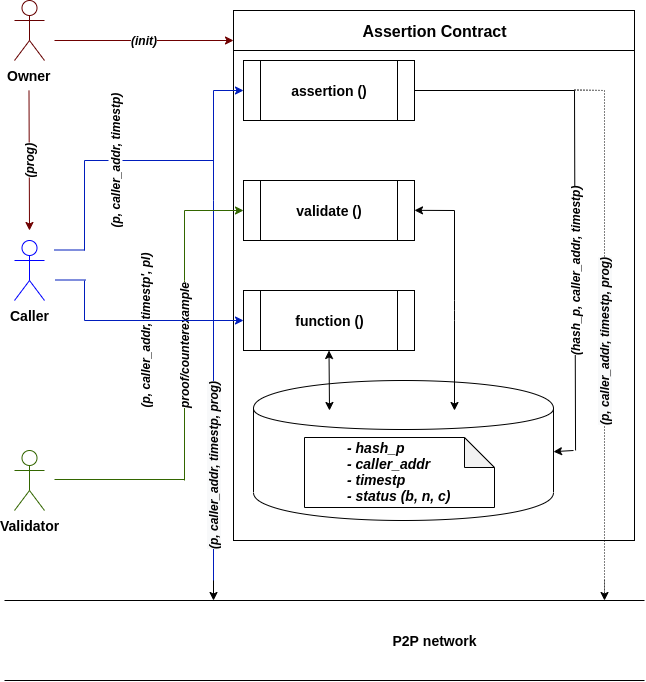
\includegraphics[scale=.6]{assertion_1}
\caption{Assertion Contract Ptotocol (1)}
\end{figure}

\subsection{Roles}
\subsubsection{Managing the contract and off-chain assertion program.}
A contract is provided by its owner on the blockchain. In addition to the code of the contract on the blockchain, there is an off-chain assertion program to find a counterexample for a submitted parameter, and this code should be available to all validators. Let us discuss two ways to distribute this off-chain assertion program.

\begin{itemize} 
\item The program code is stored inside the contract code. In this case, the code is available on the blockchain. However, it could be expensive to store the code on the blockchain, and especially impossible if the program is very large. (For discussion: and can be sent as data in a normal transfer?). 
\item The program code is stored off-chain and should always be available to callers/validators upon request. There are two ways to make it available to validators: (1) the program is stored on a source that can be accessed by the caller/validator, or the owner can make it available on request, which is sent to a caller/validator on request, and (2) when a caller invokes an assertion function, it should send the program to the network via messaging systems such as waku in eutherum, or the owner should broadcast it to the network when deplying the contract, and in this case interested validators should store the code locally. \end{itemize}



\subsubsection{Interacting with the smart contract.}
A caller must first pass the parameter to an assertion function before passing it for use in an actual code, namely a work function. The parameter is then distributed and to be checked by validators. We consider here two ways in which the call to the work function can be handled after the parameter has been validated.

\begin{itemize}
\item The work function is called by a caller after the process of checking the parameter is complete (Figure 1). There must be some restrictions on calling this function, for example, the function can be called only after the parameter has been available for verification for a certain time, or there is a fixed number of proofs (computational proof without counterexample) that the parameter has received. The main point with this method is that we do not need to store the parameter, only its hash in the storage, and the other parameters that do not need to be checked can also be submitted only when the caller invokes the work function. The caller must also transmit the timestamp when it presents the parameter for verification. With the hash of the parameter, the address of the caller and the timestamp, a search in the storage looks for the matching information and constraints to decide whether the work function should be executed or not.
\item The function is called by the validator function (Figure 2). The good thing about this method is that the process of validating the parameter and calling the normal function is not visible to the user. However, there are two arguments against this way: (1) it is necessary to store the parameter as well as others in storage, which comes at a high cost, and (2) since the function is called from the validate function, there should be a way to ensure that it is called when the parameter is valid and certain conditions are met. Also, it might be difficult to deal with timing constraints since these functions are passive. 
\end{itemize}

\paragraph{Submitting the parameter.} A caller passes the parameter to be checked by calling an assertion function. The function then stores all the necessary information, namely the parameter hash in Figure 1 (or the parameter in Figure 2), the caller's address, and the timestamp in memory as if in a record. The parameter's record also contains initial information to monitor the progress of the parameter's verification, e.g., how many computational proofs have been presented, whether a counterexample has been found, etc. This information is used to review a proof or counterexample presented by a validator, and to decide when a work function can be called for that parameter. The caller can then send this information along with the off-chain assertion program to all validators via a messaging system.

(For discussion: should the function publish this information on the blockchain via the IDM in a transfer to all examiners as this is costly?).

\paragraph{Calling a work function.}
We consider the case where the work function is called by a caller after the parameter has been checked. Thus, the caller first passes its parameter to the assertion function and then waits a while to be sure that the parameter has been checked. The record corresponding to the parameter stored in the storage is updated when a proof or counterexample is presented. After some time has passed or enough proof has been received from the validators. The caller invokes the work function with the current parameter and timestamp, which is matched against the stored parameter hash and timestamp. They must match and satisfy some other conditions, e.g., a certain amount of time must have passed and no counterexample must be found. If all requirements are met, the actual work is done and the record of the parameter is deleted from memory to relieve the storage. If no record is found that matches the input data, the actual work with the input data is not performed.


\begin{figure}
\centering
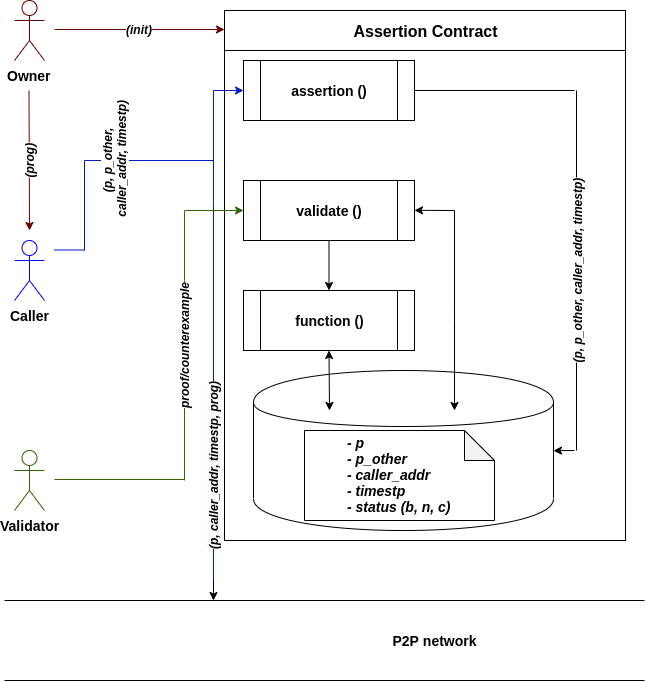
\includegraphics[scale=.6]{assertion_2}
\caption{Assertion Contract Ptotocol(2)}
\end{figure}

\subsubsection{Validating a parameter}
When a parameter is sent to an validator, the validator runs the off-chain assertion program to find a counterexample. If so, the validator submits the parameter to the blockchain to receive a reward. Otherwise, a computation proof is submitted, which should be automatically generated when the program is executed. A validator interacts with the contract in two ways: he can announce a counterexample and submit a calculation proof. The validator must clarify which parameter is being verified by submitting the parameter, the address of the caller, and the timestamp. This information is then matched with the records in the storage.

\paragraph{Submission of proof.} After running the program but finding no counterexample, the validator submits a computational proof to receive a reward for running the check. The proof should be unique for each run. Since the off-chain assertion program is the same for every validators, we need the address of the validator for each parameter to make the proof unique for each validator. This prevents the validator from copying a calculation proof from others. Also, since the proof cannot be stored in the blockchain or it would be too costly, a timestamp is added for the execution of the program to prevent an validator from using the same proof for multiple submission. Therefore, the proof should be generated from the program and is calculated based on the parameter's information provided. Each validator who runs the program enters the parameter, the address of the caller, the timestamp, and the time at which he or she runs the program, as well as his or her address. This information is used to calculate an unique computation proof.
\paragraph{Asserting a counterexample.} a validator can submit a counterexample and the counterexample is then checked by the contract on the blockchain. If it is correct, there is an award to the validator and the function updates the store accordingly. There are two options: update the status or delete the record. 
 
(For discussion: what happens if the parameter was checked but not executed by the contract caller. It will occupy the memory forever. Since a function is passive in this case, there should be a mode (function) executed by the owner to delete this parameter after some time. Also, the program is executed to check the parameter to find a counterexample. So basically it generates a random number (since it is off-chain, why do not we run the entire check - safe time) a limited number of proofs while it runs the check).

When the normal function is called by the validate function, the storage stores the parameter in place of its hash and any other parameters required for the normal function. If certain requirements are met, the function is called when a validator submits the proof.




\section{A Prototype Implementation}
\section{Cost Analysis}
\section{Related work}
\section{Conclusion}
\bibliographystyle{splncs04}
\bibliography{bio}
\end{document}


